%%
% This is an Overleaf template for presentations
% using the TUM Corporate Desing https://www.tum.de/cd
%
% For further details on how to use the template, take a look at our
% GitLab repository and browse through our test documents
% https://gitlab.lrz.de/latex4ei/tum-templates.
%
% The tumbeamer class is based on the beamer class.
% If you need further customization please consult the beamer class guide
% https://ctan.org/pkg/beamer.
% Additional class options are passed down to the base class.
%
% If you encounter any bugs or undesired behaviour, please raise an issue
% in our GitLab repository
% https://gitlab.lrz.de/latex4ei/tum-templates/issues
% and provide a description and minimal working example of your problem.
%%

%\makeatletter
%\def\input@path{{../beamer/}}
%\makeatother

\documentclass[
  german,            % define the document language (english, german)
  aspectratio=169,    % define the aspect ratio (169, 43)
  % handout=2on1,       % create handout with multiple slides (2on1, 4on1)
  % partpage=false,     % insert page at beginning of parts (true, false)
  % sectionpage=true,   % insert page at beginning of sections (true, false)
]{tumbeamer}


% load additional packages
\usepackage{booktabs}
\usepackage{graphicx}
\usepackage{tikz}
\usepackage{url}
\usepackage{pgfplots}
\usepackage{hyperref}
\usepackage{pmboxdraw}
\usepackage{float}
\usepackage{listings}
\usepackage{circuitikz}
%\usepackage[european]{circuitikz}

% image path
\graphicspath{ {./resources/} }

% presentation metadata
\title{Übung 05: Boolesche Algebra und \\kombinatorische Schaltungen}
\subtitle{Einführung in die Rechnerarchitektur}
\author{Niklas Ladurner}

\institute{\theChairName\\\theDepartmentName\\\theUniversityName}
\date[\today]{\today}

\footline{\insertauthor~|~\insertshorttitle~|~\insertshortdate}


% macro to configure the style of the presentation
\TUMbeamersetup{
  title page = TUM tower,         % style of the title page
  part page = TUM toc,            % style of part pages
  section page = TUM toc,         % style of section pages
  content page = TUM more space,  % style of normal content pages
  tower scale = 1.0,              % scaling factor of TUM tower (if used)
  headline = TUM threeliner,      % which variation of headline to use
  footline = TUM default,         % which variation of footline to use
  % configure on which pages headlines and footlines should be printed
  headline on = {title page},
  footline on = {every page, title page=false},
}

% available frame styles for title page, part page, and section page:
% TUM default, TUM tower, TUM centered,
% TUM blue default, TUM blue tower, TUM blue centered,
% TUM shaded default, TUM shaded tower, TUM shaded centered,
% TUM flags
%
% additional frame styles for part page and section page:
% TUM toc
%
% available frame styles for content pages:
% TUM default, TUM more space
%
% available headline options:
% TUM empty, TUM oneliner, TUM twoliner, TUM threeliner, TUM logothreeliner
%
% available footline options:
% TUM empty, TUM default, TUM infoline


\begin{document}

\maketitle

\begin{frame}[c]{}{}
  \begin{center}
    \LARGE  Durchzählen!
  \end{center}
\end{frame}

\begin{frame}[c]{}{}
  \begin{center}
    \LARGE  Keine Garantie für die Richtigkeit der Tutorfolien: Bei Unklarheiten/Unstimmigkeiten
    haben VL/ZÜ-Folien Recht!
  \end{center}
\end{frame}

\begin{frame}[fragile, c]{Boolesche Funktionen}{}
  \centering
  \begin{columns}[T]
    \begin{column}{0.3\textwidth}
      \centering
      OR-Gatter

      \vspace{0.2cm}

      \begin{circuitikz}
        \draw (0,0) node[ieeestd or port] (or) {};
        \draw (or.in 1) node[left] {$A$};
        \draw (or.in 2) node[left] {$B$};
        \draw (or.out) -- ++(0.5,0) node[right] {$A \lor B$};
      \end{circuitikz}

      \vspace{-0.3cm}

      \[
        \begin{array}{|c|c|c|}
          \hline
          A & B & A \lor B \\
          \hline
          0 & 0 & 0        \\
          0 & 1 & 1        \\
          1 & 0 & 1        \\
          1 & 1 & 1        \\
          \hline
        \end{array}
      \]

    \end{column}

    \begin{column}{0.3\textwidth}
      \centering
      AND-Gatter

      \vspace{0.2cm}

      \begin{circuitikz}
        \draw (0,0) node[ieeestd and port] (and) {};
        \draw (and.in 1) node[left] {$A$};
        \draw (and.in 2) node[left] {$B$};
        \draw (and.out) -- ++(0.5,0) node[right] {$A \land B$};
      \end{circuitikz}

      \vspace{-0.3cm}

      \[
        \begin{array}{|c|c|c|}
          \hline
          A & B & A \land B \\
          \hline
          0 & 0 & 0         \\
          0 & 1 & 0         \\
          1 & 0 & 0         \\
          1 & 1 & 1         \\
          \hline
        \end{array}
      \]

    \end{column}

    \begin{column}{0.3\textwidth}
      \centering
      NOT-Gatter

      \vspace{0.2cm}

      \begin{circuitikz}
        \draw (0,0) node[ieeestd not port] (not) {};
        \draw (not.in) -- ++(-0.5,0) node[left] {$A$};
        \draw (not.out) -- ++(0.5,0) node[right] {$\lnot A$};
      \end{circuitikz}

      \vspace{-0.3cm}

      \[
        \begin{array}{|c|c|}
          \hline
          A & \lnot A \\
          \hline
          0 & 1       \\
          1 & 0       \\
          \hline
        \end{array}
      \]

    \end{column}

  \end{columns}
\end{frame}

\begin{frame}[c]{Boolesche Funktionen}{}
  \begin{itemize}
    \item Alternative Schreibweisen: $x+y$ für OR, $x\cdot y$ für AND, $\overline{x}$ für NOT
    \item Gatter in europäischer Norm einfacher zu zeichnen und besser unterscheidbar $\rightarrow$\\ in Klausur einheitlich verwenden!
    \item weitere wichtige Funktionen (bekannt aus DS): $\oplus$ (XOR), $\rightarrow$ (Implikation), $\leftrightarrow$ (Bikonditional, Iff, XNOR)
    \item Funktionale Vollständigkeit: Menge $\mathcal{F}$ sodass alle boolschen Funktionen als Kombination von $f_i\in\mathcal{F}$ darstellbar sind. Beispiel: $\{\wedge, \neg\}$
  \end{itemize}
\end{frame}

\begin{frame}[c]{Gesetze der Booleschen Algebra}{}
  \begin{itemize}
    \item Identität: $x+0=x$, $x\cdot 1=x$
    \item Idempotenz: $x+x=x$, $x\cdot x=x$
    \item Komplementärgesetz: $x+\overline{x}=1$, $x\cdot\overline{x}=0$
    \item Involution: $\overline{\overline{x}}=x$
    \item De Morgan: $\overline{x+y}=\overline{x}\cdot\overline{y}$ und $\overline{x\cdot y}=\overline{x}+\overline{y}$
    \item Absorption: $x+(x\cdot y)=x$, $x\cdot(x+y)=x$
    \item Distributivität: $x\cdot(y+z)=(x\cdot y)+ (x\cdot z)$ und $x+(y\cdot z)=(x+y)\cdot (x+z)$
  \end{itemize}
\end{frame}

\begin{frame}[c]{Normalformen}{}
  \begin{itemize}
    \item Konjunktive Normalform (OR in den Klammern, AND dazwischen): $(x+y) \cdot (x+\overline{y})$
    \item Disjunktive Normalform (AND in den Klammern, OR dazwischen): $(x\cdot y) + (x\cdot\overline{y})$
  \end{itemize}
  \centering
  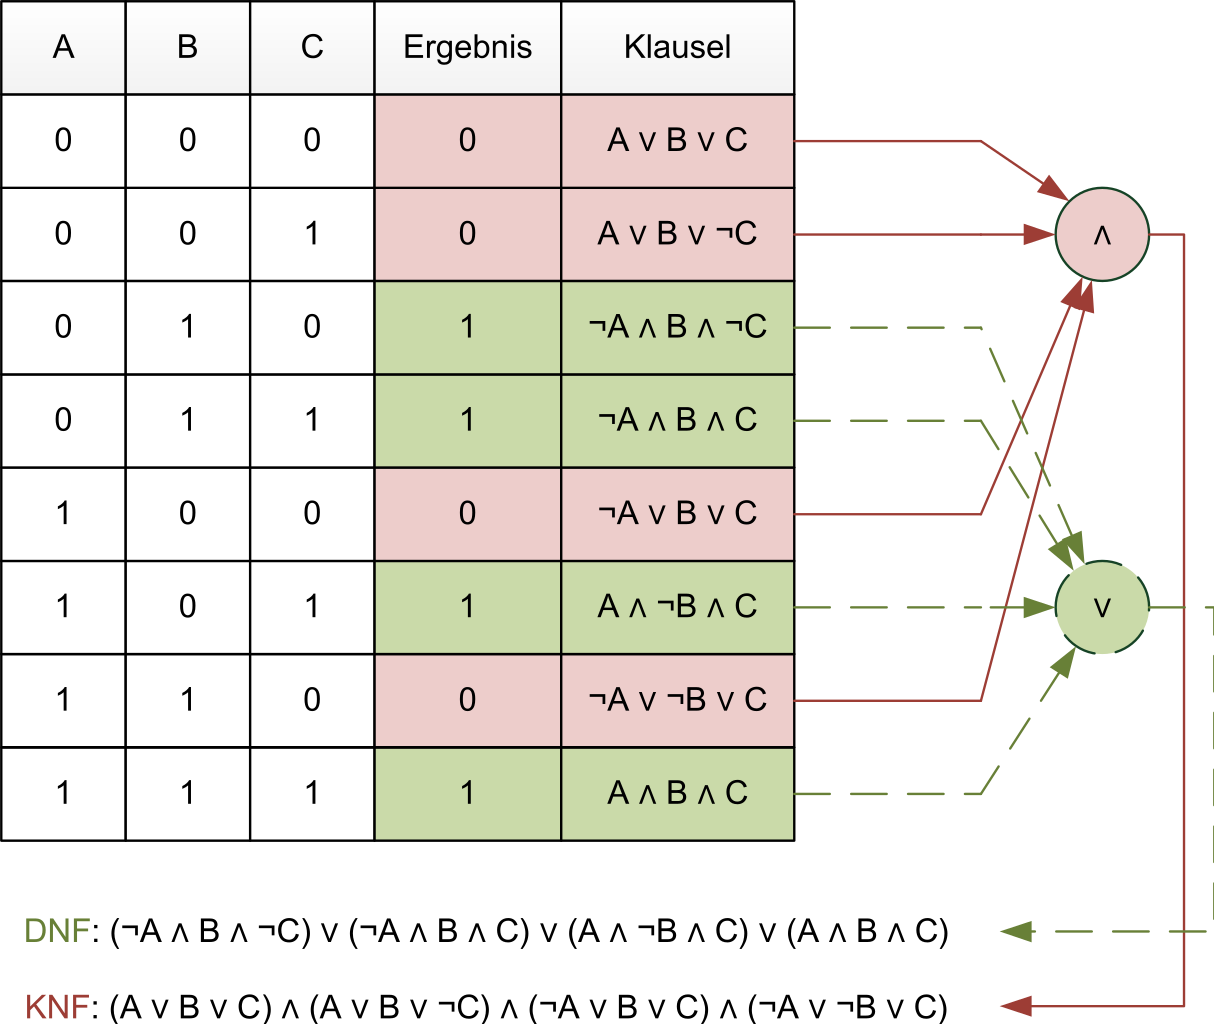
\includegraphics[height=0.70\textheight]{resources/w05_knf_dnf}
\end{frame}

\begin{frame}[c]{}{}
  \begin{center}
    \LARGE Fragen?
  \end{center}
\end{frame}

\begin{frame}[c]{Artemis-Hausaufgaben}{}
  \begin{itemize}
    \item H05 - Wasserstandskontrolle bis 26.11.2023 23:59 Uhr
    \item Wahrheitstabelle, boolsche Funktion und Schaltung in Logisim
  \end{itemize}
\end{frame}

\begin{frame}[fragile, c]{Links}{}
  \begin{itemize}
    \item Zulip: \href{https://zulip.in.tum.de/#narrow/stream/1917-ERA-Tutorium---Mi-1600-MI4}{\glqq ERA Tutorium - Mi-1600-MI4\grqq}
          bzw. \href{https://zulip.in.tum.de/#narrow/stream/1940-ERA-Tutorium---Fr-1100-MW2}{\glqq ERA Tutorium - Fr-1100-MW2\grqq}
    \item \href{https://www.elektronik-kompendium.de/sites/dig/2609191.htm}{Logische Grundschaltungen}
    \item \href{https://www.elektronik-kompendium.de/sites/dig/0209031.htm}{Halb- und Volladdierer}
    \item \href{https://github.com/logisim-evolution/logisim-evolution/releases}{Logisim Evolution}
    \item \href{https://www.biancahoegel.de/logik/normalform_konjunktiv.html}{Konjunktive Normalform}
  \end{itemize}
\end{frame}

\maketitle

\end{document}
